\documentclass{article}\usepackage[]{graphicx}\usepackage[]{color}
%% maxwidth is the original width if it is less than linewidth
%% otherwise use linewidth (to make sure the graphics do not exceed the margin)
\makeatletter
\def\maxwidth{ %
  \ifdim\Gin@nat@width>\linewidth
    \linewidth
  \else
    \Gin@nat@width
  \fi
}
\makeatother

\definecolor{fgcolor}{rgb}{0.345, 0.345, 0.345}
\newcommand{\hlnum}[1]{\textcolor[rgb]{0.686,0.059,0.569}{#1}}%
\newcommand{\hlstr}[1]{\textcolor[rgb]{0.192,0.494,0.8}{#1}}%
\newcommand{\hlcom}[1]{\textcolor[rgb]{0.678,0.584,0.686}{\textit{#1}}}%
\newcommand{\hlopt}[1]{\textcolor[rgb]{0,0,0}{#1}}%
\newcommand{\hlstd}[1]{\textcolor[rgb]{0.345,0.345,0.345}{#1}}%
\newcommand{\hlkwa}[1]{\textcolor[rgb]{0.161,0.373,0.58}{\textbf{#1}}}%
\newcommand{\hlkwb}[1]{\textcolor[rgb]{0.69,0.353,0.396}{#1}}%
\newcommand{\hlkwc}[1]{\textcolor[rgb]{0.333,0.667,0.333}{#1}}%
\newcommand{\hlkwd}[1]{\textcolor[rgb]{0.737,0.353,0.396}{\textbf{#1}}}%
\let\hlipl\hlkwb

\usepackage{framed}
\makeatletter
\newenvironment{kframe}{%
 \def\at@end@of@kframe{}%
 \ifinner\ifhmode%
  \def\at@end@of@kframe{\end{minipage}}%
  \begin{minipage}{\columnwidth}%
 \fi\fi%
 \def\FrameCommand##1{\hskip\@totalleftmargin \hskip-\fboxsep
 \colorbox{shadecolor}{##1}\hskip-\fboxsep
     % There is no \\@totalrightmargin, so:
     \hskip-\linewidth \hskip-\@totalleftmargin \hskip\columnwidth}%
 \MakeFramed {\advance\hsize-\width
   \@totalleftmargin\z@ \linewidth\hsize
   \@setminipage}}%
 {\par\unskip\endMakeFramed%
 \at@end@of@kframe}
\makeatother

\definecolor{shadecolor}{rgb}{.97, .97, .97}
\definecolor{messagecolor}{rgb}{0, 0, 0}
\definecolor{warningcolor}{rgb}{1, 0, 1}
\definecolor{errorcolor}{rgb}{1, 0, 0}
\newenvironment{knitrout}{}{} % an empty environment to be redefined in TeX

\usepackage{alltt}

% \usepackage[utf8]{inputenc}
\usepackage{amsmath}
\usepackage{fancyhdr}
\usepackage{array}
\usepackage{longtable}
\usepackage{graphicx}
\usepackage{color}
\usepackage[letterpaper, margin=1in]{geometry}
\usepackage{lscape}
\newcommand{\blandscape}{\begin{landscape}}
\newcommand{\elandscape}{\end{landscape}}
\usepackage{dcolumn}
\usepackage{bbm}
\usepackage{threeparttable}
\usepackage{booktabs}
\usepackage{expex}
\usepackage{pdflscape}
\usepackage{rotating, graphicx}
\usepackage{tabulary}
\usepackage{lscape}
\usepackage{makecell}
\usepackage{algorithm}
\usepackage{multirow}
\usepackage{colortbl}
\usepackage{longtable}
\usepackage{array}
\usepackage{multirow}
\usepackage{wrapfig}
\usepackage{float}
\usepackage{pdflscape}
\usepackage{tabu}
\usepackage{threeparttable}

\title{%
Homework 3\\
\large Applied Mutlivariate Analysis}
\date{September 22, 2018}
\author{Emorie Beck}
\IfFileExists{upquote.sty}{\usepackage{upquote}}{}
\begin{document}
\maketitle
% \SweaveOpts{concordance=TRUE}

\section{Workspace}
\subsection{Packages}



\begin{knitrout}
\definecolor{shadecolor}{rgb}{0.969, 0.969, 0.969}\color{fgcolor}\begin{kframe}
\begin{alltt}
\hlkwd{library}\hlstd{(car)}
\hlkwd{library}\hlstd{(knitr)}
\hlkwd{library}\hlstd{(psych)}
\hlkwd{library}\hlstd{(lavaan)}
\hlkwd{library}\hlstd{(semPlot)}
\hlkwd{library}\hlstd{(kableExtra)}
\hlkwd{library}\hlstd{(multcomp)}
\hlkwd{library}\hlstd{(lme4)}
\hlkwd{library}\hlstd{(plyr)}
\hlkwd{library}\hlstd{(tidyverse)}
\hlkwd{library}\hlstd{(MVN)}
\end{alltt}
\end{kframe}
\end{knitrout}



\subsection{data}
The file, Set\_5.csv, contains data from a study in which college students completed the NEO-PI Personality Inventory. This 240-item scale purportedly measures the Big Five personality dimensions, assumed to be fairly independent. The inventory is scored on 6 subscales per dimension, listed below. The file contains the subscale scores, rather than the individual items, which should help reduce the impact of the small sample size.\\

Neuroticism: Anxiety\\
Neuroticism: Angry\_Hostility\\
Neuroticism: Depression\\
Neuroticism: Self\_Consciousness\\
Neuroticism: Impulsiveness\\
Neuroticism: Vulnerability\\
Extraversion: Warmth\\
Extraversion: Gregariousness\\
Extraversion: Assertiveness\\
Extraversion: Activity\\
Extraversion: Excitement\_Seeking\\
Extraversion: Positive\_Emotions\\
Openness: Fantasy\\
Openness: Aesthetics\\
Openness: Feelings\\
Openness: Actions\\
Openness: Ideas\\
Openness: Values\\
Agreeableness: Trust\\
Agreeableness: Straightforwardness \\
Agreeableness: Altruism\\
Agreeableness: Compliance\\
Agreeableness: Modesty\\
Agreeableness: Tender\_Mindedness\\
Conscientiousness: Competence\\
Conscientiousness: Order\\
Conscientiousness: Dutifulness\\
Conscientiousness: Achievement\_Striving \\
Conscientiousness: Self\_Discipline\\
Conscientiousness: Deliberation\\

\begin{knitrout}
\definecolor{shadecolor}{rgb}{0.969, 0.969, 0.969}\color{fgcolor}\begin{kframe}
\begin{alltt}
\hlstd{wd} \hlkwb{<-} \hlstr{"https://github.com/emoriebeck/homeworks/raw/master/multivariate/homeworks/homework6"}

\hlstd{dat} \hlkwb{<-} \hlkwd{sprintf}\hlstd{(}\hlstr{"%s/Set_5(1).csv"}\hlstd{, wd)} \hlopt
  \hlkwd{read.csv}\hlstd{(.,} \hlkwc{stringsAsFactors} \hlstd{= F)}

\hlkwd{head}\hlstd{(dat)}
\end{alltt}
\begin{verbatim}
##   ID Anxiety Angry_Hostility Depression Self_Consciousness Impulsiveness
## 1  2   2.625           2.000      1.750           2.250000         2.625
## 2  3   3.625           2.875      3.000           3.500000         4.250
## 3  4   3.000           2.750      2.625           2.875000         3.000
## 4  5   4.375           3.125      4.500           4.000000         3.875
## 5  6   3.500           2.875      3.000           2.571429         3.625
## 6  7   4.000           4.125      2.875           2.375000         4.000
##   Vulnerability   Warmth Gregariousness Assertiveness Activity
## 1      2.166667 4.666667          4.000      3.000000 4.833333
## 2      2.125000 4.500000          2.750      2.625000 3.000000
## 3      2.875000 3.750000          3.125      2.375000 3.250000
## 4      3.750000 3.250000          2.250      2.500000 1.875000
## 5      2.750000 3.750000          3.125      3.285714 3.500000
## 6      3.125000 3.500000          2.625      3.375000 3.125000
##   Excitement_Seeking Positive_Emotions  Fantasy Aesthetics Feelings
## 1              3.500             4.750 3.857143   3.571429 4.666667
## 2              2.875             3.500 3.500000   4.125000 3.625000
## 3              3.875             3.375 3.375000   3.500000 3.250000
## 4              2.750             2.625 3.000000   3.750000 4.250000
## 5              3.750             3.625 3.125000   1.625000 3.125000
## 6              2.000             3.375 3.500000   2.000000 3.250000
##    Actions Ideas Values Trust Straightforwardness Altruism Compliance
## 1 2.571429 4.400  4.600 5.000            2.166667 4.833333      2.750
## 2 3.000000 3.875  3.125 3.250            3.750000 3.625000      3.125
## 3 2.375000 4.125  3.500 3.250            3.125000 4.000000      3.750
## 4 3.375000 2.750  4.125 3.000            3.428571 3.875000      4.000
## 5 2.750000 2.500  3.625 3.375            3.250000 4.125000      3.625
## 6 2.625000 1.125  3.625 2.500            2.875000 3.000000      2.250
##   Modesty Tender_Mindedness Competence Order Dutifulness
## 1   4.000          3.833333       4.50 3.625    3.285714
## 2   2.625          3.250000       3.00 2.250    3.875000
## 3   2.750          3.250000       3.75 3.250    3.750000
## 4   4.125          3.750000       2.75 3.000    2.875000
## 5   3.375          3.375000       3.75 4.000    3.750000
## 6   2.625          3.375000       3.00 3.625    2.625000
##   Achievement_Striving Self_Discipline Deliberation
## 1             4.333333           4.250        2.875
## 2             2.750000           3.750        3.500
## 3             3.375000           3.375        3.125
## 4             2.875000           2.625        3.250
## 5             3.375000           2.875        3.375
## 6             3.000000           2.625        2.625
\end{verbatim}
\end{kframe}
\end{knitrout}

\begin{knitrout}
\definecolor{shadecolor}{rgb}{0.969, 0.969, 0.969}\color{fgcolor}\begin{kframe}
\begin{alltt}
\hlstd{source} \hlkwb{<-} \hlkwd{tribble}\hlstd{(}
\hlopt{~}\hlstd{Factor,} \hlopt{~}\hlstd{Facet,}
\hlstr{"Neuroticism"}\hlstd{,} \hlstr{"Anxiety"}\hlstd{,}
\hlstr{"Neuroticism"}\hlstd{,} \hlstr{"Angry_Hostility"}\hlstd{,}
\hlstr{"Neuroticism"}\hlstd{,} \hlstr{"Depression"}\hlstd{,}
\hlstr{"Neuroticism"}\hlstd{,} \hlstr{"Self_Consciousness"}\hlstd{,}
\hlstr{"Neuroticism"}\hlstd{,} \hlstr{"Impulsiveness"}\hlstd{,}
\hlstr{"Neuroticism"}\hlstd{,} \hlstr{"Vulnerability"}\hlstd{,}
\hlstr{"Extraversion"}\hlstd{,} \hlstr{"Warmth"}\hlstd{,}
\hlstr{"Extraversion"}\hlstd{,} \hlstr{"Gregariousness"}\hlstd{,}
\hlstr{"Extraversion"}\hlstd{,} \hlstr{"Assertiveness"}\hlstd{,}
\hlstr{"Extraversion"}\hlstd{,} \hlstr{"Activity"}\hlstd{,}
\hlstr{"Extraversion"}\hlstd{,} \hlstr{"Excitement_Seeking"}\hlstd{,}
\hlstr{"Extraversion"}\hlstd{,} \hlstr{"Positive_Emotions"}\hlstd{,}
\hlstr{"Openness"}\hlstd{,} \hlstr{"Fantasy"}\hlstd{,}
\hlstr{"Openness"}\hlstd{,} \hlstr{"Aesthetics"}\hlstd{,}
\hlstr{"Openness"}\hlstd{,} \hlstr{"Feelings"}\hlstd{,}
\hlstr{"Openness"}\hlstd{,} \hlstr{"Actions"}\hlstd{,}
\hlstr{"Openness"}\hlstd{,} \hlstr{"Ideas"}\hlstd{,}
\hlstr{"Openness"}\hlstd{,} \hlstr{"Values"}\hlstd{,}
\hlstr{"Agreeableness"}\hlstd{,} \hlstr{"Trust"}\hlstd{,}
\hlstr{"Agreeableness"}\hlstd{,} \hlstr{"Straightforwardness"} \hlstd{,}
\hlstr{"Agreeableness"}\hlstd{,} \hlstr{"Altruism"}\hlstd{,}
\hlstr{"Agreeableness"}\hlstd{,} \hlstr{"Compliance"}\hlstd{,}
\hlstr{"Agreeableness"}\hlstd{,} \hlstr{"Modesty"}\hlstd{,}
\hlstr{"Agreeableness"}\hlstd{,} \hlstr{"Tender_Mindedness"}\hlstd{,}
\hlstr{"Conscientiousness"}\hlstd{,} \hlstr{"Competence"}\hlstd{,}
\hlstr{"Conscientiousness"}\hlstd{,} \hlstr{"Order"}\hlstd{,}
\hlstr{"Conscientiousness"}\hlstd{,} \hlstr{"Dutifulness"}\hlstd{,}
\hlstr{"Conscientiousness"}\hlstd{,} \hlstr{"Achievement_Striving"}\hlstd{,}
\hlstr{"Conscientiousness"}\hlstd{,} \hlstr{"Self_Discipline"}\hlstd{,}
\hlstr{"Conscientiousness"}\hlstd{,} \hlstr{"Deliberation"}
\hlstd{)}

\hlstd{dat} \hlkwb{<-} \hlstd{dat} \hlopt \hlkwd{select}\hlstd{(ID, source}\hlopt{$}\hlstd{Facet)}
\end{alltt}
\end{kframe}
\end{knitrout}



Use confirmatory factor analysis to answer the following questions.  

\section{Question 1}
First, test the hypothesis that the structure of personality is best described by five independent factors. How well does this model fit the data? Base your decision on the $\chi^2$ goodness of fit test along with the goodness-of-fit index of your choice.  
\begin{knitrout}
\definecolor{shadecolor}{rgb}{0.969, 0.969, 0.969}\color{fgcolor}\begin{kframe}
\begin{alltt}
\hlstd{b5.base} \hlkwb{<-} \hlstr{'
# define the measurement model
E =~ Warmth + Gregariousness + Assertiveness + Activity + Excitement_Seeking + Positive_Emotions
A =~ Trust + Straightforwardness + Altruism + Compliance + Modesty + Tender_Mindedness
C =~ Competence + Order + Dutifulness + Competence + Order + Dutifulness
N =~ Anxiety + Angry_Hostility + Depression + Self_Consciousness + Impulsiveness + Vulnerability
O =~ Fantasy + Aesthetics + Feelings + Actions + Ideas + Values
'}
\hlstd{b5.uncorr} \hlkwb{<-}
\hlstr{'
# uncorrelated factors
E ~~ 0*A
E ~~ 0*C
E ~~ 0*N
E ~~ 0*O

A ~~ 0*C
A ~~ 0*N
A ~~ 0*O

C ~~ 0*N
C ~~ 0*O
'}

\hlstd{b5.mod} \hlkwb{<-} \hlkwd{paste}\hlstd{(b5.base,} \hlstr{'\textbackslash{}n\textbackslash{}n'}\hlstd{, b5.uncorr,} \hlkwc{sep} \hlstd{=} \hlstr{''}\hlstd{,} \hlkwc{collapse} \hlstd{=} \hlstr{''}\hlstd{)}

\hlstd{fit1} \hlkwb{<-} \hlkwd{cfa}\hlstd{(b5.mod, dat,} \hlkwc{orthogonal} \hlstd{= T,} \hlkwc{missing} \hlstd{=} \hlstr{'ML'}\hlstd{,} \hlkwc{std.lv} \hlstd{= T)}

\hlkwd{semPaths}\hlstd{(fit1,} \hlkwc{layout} \hlstd{=} \hlstr{"circle2"}\hlstd{)}
\end{alltt}
\end{kframe}
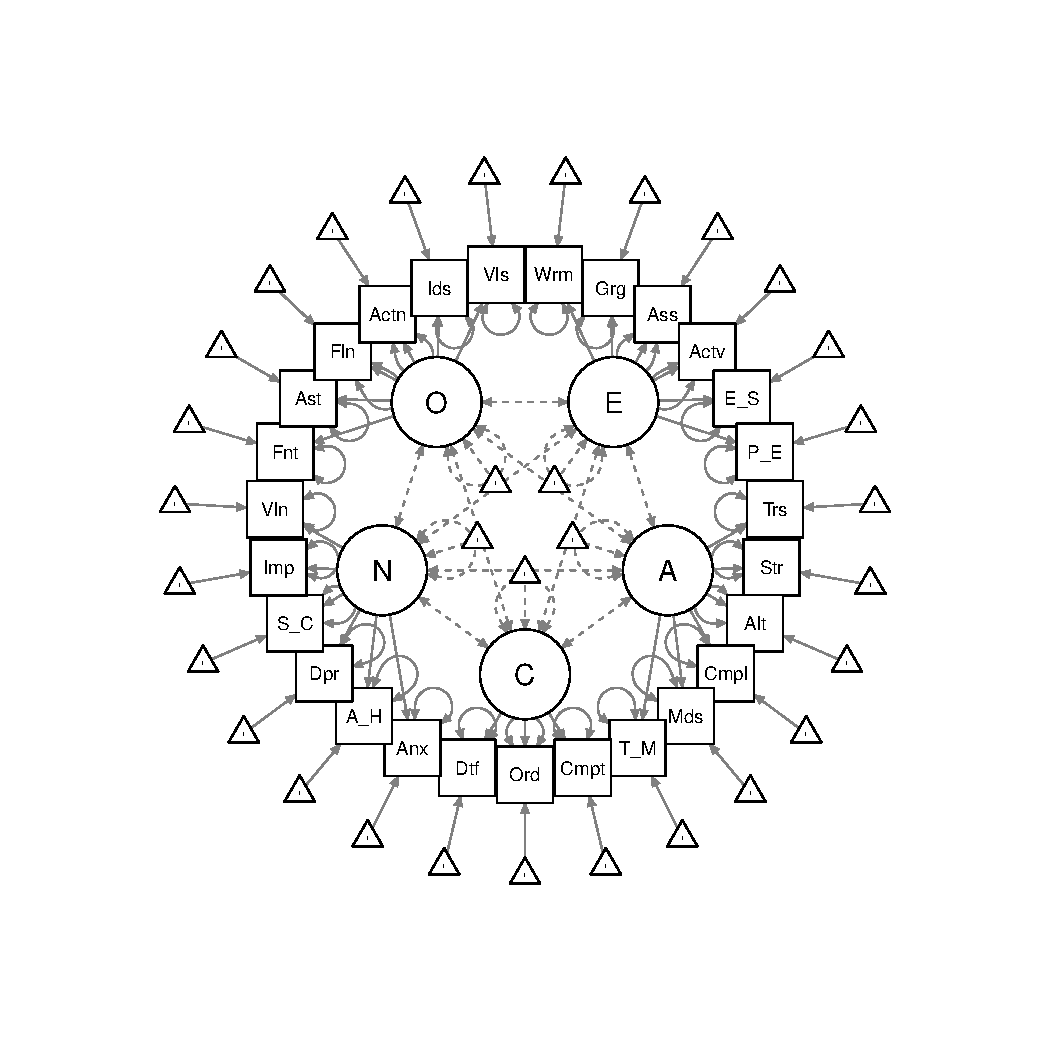
\includegraphics[width=\maxwidth]{figure/unnamed-chunk-5-1} 
\begin{kframe}\begin{alltt}
\hlkwd{summary}\hlstd{(fit1)}
\end{alltt}
\begin{verbatim}
## lavaan 0.6-3 ended normally after 36 iterations
## 
##   Optimization method                           NLMINB
##   Number of free parameters                         81
## 
##   Number of observations                           201
##   Number of missing patterns                         1
## 
##   Estimator                                         ML
##   Model Fit Test Statistic                    1467.470
##   Degrees of freedom                               324
##   P-value (Chi-square)                           0.000
## 
## Parameter Estimates:
## 
##   Information                                 Observed
##   Observed information based on                Hessian
##   Standard Errors                             Standard
## 
## Latent Variables:
##                    Estimate  Std.Err  z-value  P(>|z|)
##   E =~                                                
##     Warmth            0.532    0.041   13.008    0.000
##     Gregariousness    0.561    0.049   11.552    0.000
##     Assertiveness     0.419    0.049    8.561    0.000
##     Activity          0.367    0.039    9.437    0.000
##     Excitemnt_Skng    0.338    0.044    7.675    0.000
##     Positive_Emtns    0.583    0.046   12.636    0.000
##   A =~                                                
##     Trust             0.461    0.048    9.600    0.000
##     Strghtfrwrdnss    0.423    0.049    8.579    0.000
##     Altruism          0.444    0.039   11.363    0.000
##     Compliance        0.417    0.044    9.443    0.000
##     Modesty           0.339    0.047    7.182    0.000
##     Tender_Mnddnss    0.343    0.038    9.149    0.000
##   C =~                                                
##     Competence        0.462    0.042   10.929    0.000
##     Order             0.499    0.052    9.571    0.000
##     Dutifulness       0.529    0.045   11.676    0.000
##   N =~                                                
##     Anxiety           0.659    0.046   14.414    0.000
##     Angry_Hostilty    0.373    0.047    7.951    0.000
##     Depression        0.719    0.049   14.696    0.000
##     Self_Conscsnss    0.518    0.041   12.666    0.000
##     Impulsiveness     0.280    0.041    6.749    0.000
##     Vulnerability     0.547    0.041   13.426    0.000
##   O =~                                                
##     Fantasy           0.515    0.050   10.399    0.000
##     Aesthetics        0.565    0.060    9.456    0.000
##     Feelings          0.384    0.046    8.337    0.000
##     Actions           0.370    0.041    9.014    0.000
##     Ideas             0.425    0.056    7.633    0.000
##     Values            0.387    0.039    9.964    0.000
## 
## Covariances:
##                    Estimate  Std.Err  z-value  P(>|z|)
##   E ~~                                                
##     A                 0.000                           
##     C                 0.000                           
##     N                 0.000                           
##     O                 0.000                           
##   A ~~                                                
##     C                 0.000                           
##     N                 0.000                           
##     O                 0.000                           
##   C ~~                                                
##     N                 0.000                           
##     O                 0.000                           
##   N ~~                                                
##     O                 0.000                           
## 
## Intercepts:
##                    Estimate  Std.Err  z-value  P(>|z|)
##    .Warmth            3.780    0.046   81.414    0.000
##    .Gregariousness    3.158    0.053   59.420    0.000
##    .Assertiveness     2.942    0.050   58.547    0.000
##    .Activity          3.229    0.041   79.567    0.000
##    .Excitemnt_Skng    3.585    0.044   81.244    0.000
##    .Positive_Emtns    3.684    0.052   70.972    0.000
##    .Trust             3.343    0.049   68.025    0.000
##    .Strghtfrwrdnss    3.248    0.049   66.111    0.000
##    .Altruism          3.897    0.041   94.212    0.000
##    .Compliance        3.115    0.045   69.344    0.000
##    .Modesty           3.161    0.046   69.056    0.000
##    .Tender_Mnddnss    3.511    0.038   92.408    0.000
##    .Competence        3.486    0.043   81.607    0.000
##    .Order             3.166    0.053   60.204    0.000
##    .Dutifulness       3.630    0.046   79.166    0.000
##    .Anxiety           3.384    0.055   61.832    0.000
##    .Angry_Hostilty    2.822    0.048   58.204    0.000
##    .Depression        2.950    0.059   49.965    0.000
##    .Self_Conscsnss    3.111    0.047   66.263    0.000
##    .Impulsiveness     3.250    0.042   77.572    0.000
##    .Vulnerability     2.610    0.048   54.699    0.000
##    .Fantasy           3.660    0.051   71.597    0.000
##    .Aesthetics        3.364    0.060   55.771    0.000
##    .Feelings          3.887    0.046   85.292    0.000
##    .Actions           2.971    0.041   72.190    0.000
##    .Ideas             3.514    0.054   64.885    0.000
##    .Values            3.784    0.040   94.948    0.000
##     E                 0.000                           
##     A                 0.000                           
##     C                 0.000                           
##     N                 0.000                           
##     O                 0.000                           
## 
## Variances:
##                    Estimate  Std.Err  z-value  P(>|z|)
##    .Warmth            0.151    0.022    6.925    0.000
##    .Gregariousness    0.254    0.032    7.901    0.000
##    .Assertiveness     0.332    0.036    9.153    0.000
##    .Activity          0.196    0.022    8.847    0.000
##    .Excitemnt_Skng    0.277    0.030    9.304    0.000
##    .Positive_Emtns    0.202    0.028    7.235    0.000
##    .Trust             0.273    0.033    8.214    0.000
##    .Strghtfrwrdnss    0.306    0.036    8.608    0.000
##    .Altruism          0.147    0.021    6.881    0.000
##    .Compliance        0.232    0.028    8.258    0.000
##    .Modesty           0.306    0.034    9.112    0.000
##    .Tender_Mnddnss    0.172    0.020    8.450    0.000
##    .Competence        0.153    0.026    5.971    0.000
##    .Order             0.306    0.039    7.878    0.000
##    .Dutifulness       0.142    0.031    4.665    0.000
##    .Anxiety           0.168    0.024    6.937    0.000
##    .Angry_Hostilty    0.333    0.035    9.563    0.000
##    .Depression        0.183    0.027    6.750    0.000
##    .Self_Conscsnss    0.175    0.021    8.279    0.000
##    .Impulsiveness     0.274    0.028    9.709    0.000
##    .Vulnerability     0.159    0.020    7.950    0.000
##    .Fantasy           0.260    0.035    7.489    0.000
##    .Aesthetics        0.412    0.051    8.074    0.000
##    .Feelings          0.270    0.031    8.699    0.000
##    .Actions           0.204    0.024    8.372    0.000
##    .Ideas             0.409    0.046    8.914    0.000
##    .Values            0.169    0.021    7.873    0.000
##     E                 1.000                           
##     A                 1.000                           
##     C                 1.000                           
##     N                 1.000                           
##     O                 1.000
\end{verbatim}
\begin{alltt}
\hlstd{fm} \hlkwb{<-} \hlkwd{fitmeasures}\hlstd{(fit1)}
\end{alltt}
\end{kframe}
\end{knitrout}

The $\chi^2$ test indicates poor model fit, $\chi^2(324) = 1467.47, p = 0$. 


\section{Question 2}
Now allow the factors to correlate.  

\subsection{Part A}
Does this model fit the data significantly better? Use a $\chi^2$ difference test to answer the question.

\begin{knitrout}
\definecolor{shadecolor}{rgb}{0.969, 0.969, 0.969}\color{fgcolor}\begin{kframe}
\begin{alltt}
\hlstd{fit2} \hlkwb{<-} \hlkwd{cfa}\hlstd{(b5.base, dat,} \hlkwc{missing} \hlstd{=} \hlstr{'ML'}\hlstd{,} \hlkwc{std.lv} \hlstd{= T)}
\hlkwd{semPaths}\hlstd{(fit2,} \hlkwc{layout} \hlstd{=} \hlstr{"circle2"}\hlstd{)}
\end{alltt}
\end{kframe}
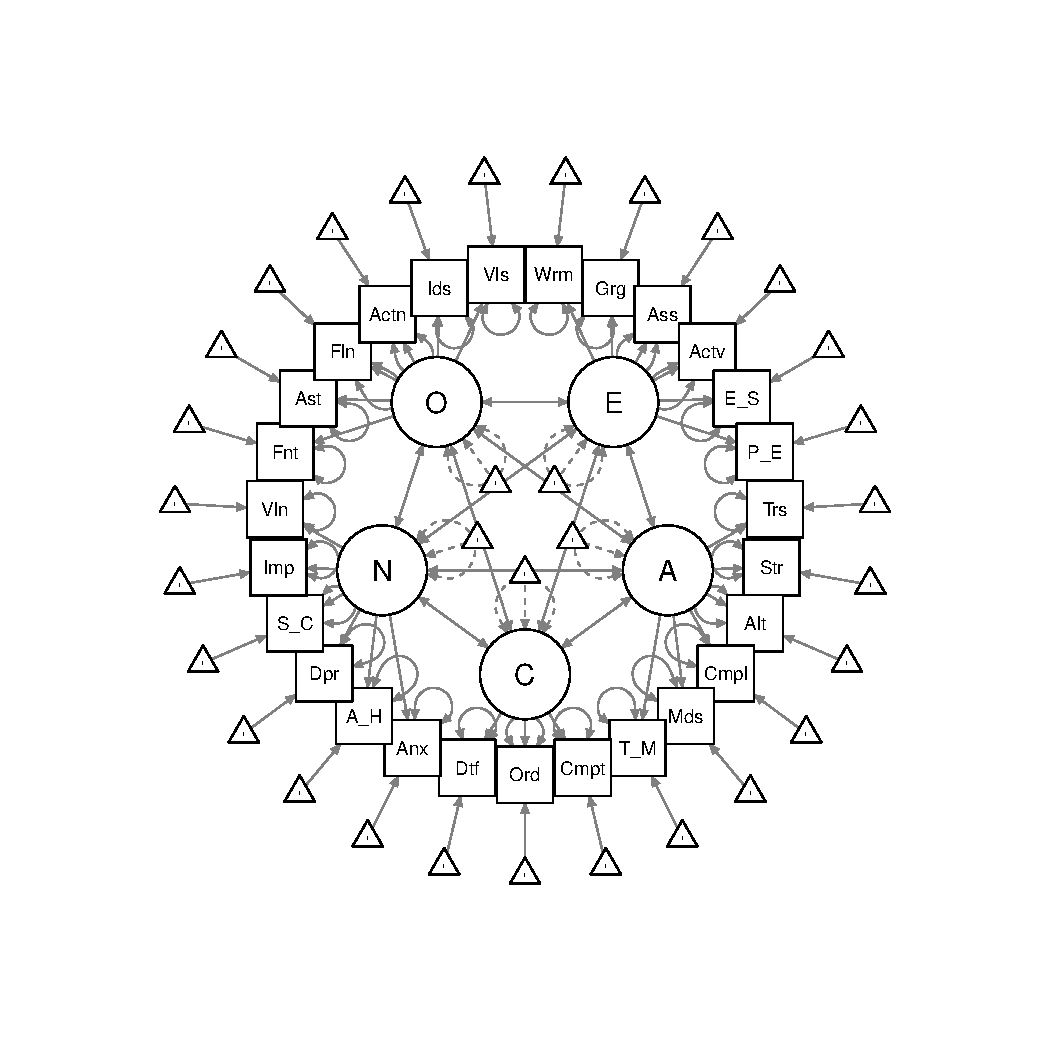
\includegraphics[width=\maxwidth]{figure/unnamed-chunk-6-1} 
\begin{kframe}\begin{alltt}
\hlstd{(c1} \hlkwb{<-} \hlkwd{anova}\hlstd{(fit1, fit2))}
\end{alltt}
\begin{verbatim}
## Chi Square Difference Test
## 
##       Df    AIC    BIC  Chisq Chisq diff Df diff Pr(>Chisq)    
## fit2 314 9196.4 9497.0 1224.6                                  
## fit1 324 9419.2 9686.8 1467.5     242.88      10  < 2.2e-16 ***
## ---
## Signif. codes:  0 '***' 0.001 '**' 0.01 '*' 0.05 '.' 0.1 ' ' 1
\end{verbatim}
\end{kframe}
\end{knitrout}

The correlated factor model fits the data better, $\chi^2_{diff}(10) = 242.88$. 

\subsection{Part B}
Which of the factor correlations are statistically significant?  
\begin{knitrout}
\definecolor{shadecolor}{rgb}{0.969, 0.969, 0.969}\color{fgcolor}\begin{kframe}
\begin{alltt}
\hlstd{res2} \hlkwb{<-} \hlkwd{parameterestimates}\hlstd{(fit2,} \hlkwc{standardized} \hlstd{= T)}

\hlstd{res2} \hlopt \hlstd{tbl_df} \hlopt
  \hlkwd{filter}\hlstd{(op} \hlopt{==} \hlstr{"~~"} \hlopt{&} \hlstd{lhs} \hlopt \hlkwd{c}\hlstd{(}\hlstr{"E"}\hlstd{,} \hlstr{"A"}\hlstd{,} \hlstr{"C"}\hlstd{,} \hlstr{"N"}\hlstd{,} \hlstr{"O"}\hlstd{))} \hlopt
  \hlkwd{full_join}\hlstd{(}\hlkwd{crossing}\hlstd{(}\hlkwc{lhs} \hlstd{=} \hlkwd{c}\hlstd{(}\hlstr{"E"}\hlstd{,} \hlstr{"A"}\hlstd{,} \hlstr{"C"}\hlstd{,} \hlstr{"N"}\hlstd{,} \hlstr{"O"}\hlstd{),} \hlkwc{rhs} \hlstd{=} \hlkwd{c}\hlstd{(}\hlstr{"E"}\hlstd{,} \hlstr{"A"}\hlstd{,} \hlstr{"C"}\hlstd{,} \hlstr{"N"}\hlstd{,} \hlstr{"O"}\hlstd{)))} \hlopt
  \hlkwd{mutate}\hlstd{(}\hlkwc{sig} \hlstd{=} \hlkwd{ifelse}\hlstd{(pvalue} \hlopt{<} \hlnum{.05}\hlstd{,} \hlstr{"sig"}\hlstd{,} \hlstr{"ns"}\hlstd{))} \hlopt
  \hlkwd{select}\hlstd{(lhs, rhs, est, ci.lower, ci.upper, sig)} \hlopt
  \hlkwd{mutate_at}\hlstd{(}\hlkwd{vars}\hlstd{(est}\hlopt{:}\hlstd{ci.upper),} \hlkwd{funs}\hlstd{(}\hlkwd{sprintf}\hlstd{(}\hlstr{"%.2f"}\hlstd{, .)))} \hlopt
  \hlkwd{mutate_at}\hlstd{(}\hlkwd{vars}\hlstd{(lhs, rhs),} \hlkwd{funs}\hlstd{(}\hlkwd{factor}\hlstd{(.,} \hlkwc{levels} \hlstd{=} \hlkwd{c}\hlstd{(}\hlstr{"E"}\hlstd{,} \hlstr{"A"}\hlstd{,} \hlstr{"C"}\hlstd{,} \hlstr{"N"}\hlstd{,} \hlstr{"O"}\hlstd{))))} \hlopt
  \hlkwd{mutate}\hlstd{(}\hlkwc{value} \hlstd{=} \hlkwd{sprintf}\hlstd{(}\hlstr{"%s [%s, %s]"}\hlstd{, est, ci.lower, ci.upper),}
         \hlkwc{value} \hlstd{=} \hlkwd{ifelse}\hlstd{(sig} \hlopt{==} \hlstr{"sig"}\hlstd{,} \hlkwd{sprintf}\hlstd{(}\hlstr{"\textbackslash{}\textbackslash{}textbf\{%s\}"}\hlstd{, value), value),}
         \hlkwc{value} \hlstd{=} \hlkwd{ifelse}\hlstd{(}\hlkwd{is.na}\hlstd{(value),} \hlstr{""}\hlstd{, value))} \hlopt
  \hlkwd{select}\hlstd{(lhs, rhs, value)} \hlopt
  \hlkwd{spread}\hlstd{(}\hlkwc{key} \hlstd{= rhs,} \hlkwc{value} \hlstd{= value)} \hlopt
  \hlkwd{kable}\hlstd{(.,} \hlstr{"latex"}\hlstd{,} \hlkwc{booktabs} \hlstd{= T,} \hlkwc{escape} \hlstd{= F,}
        \hlkwc{caption} \hlstd{=} \hlstr{"Question 2B"}\hlstd{)} \hlopt
  \hlkwd{kable_styling}\hlstd{(}\hlkwc{full_width} \hlstd{= F)}
\end{alltt}
\end{kframe}\begin{table}

\caption{\label{tab:unnamed-chunk-7}Question 2B}
\centering
\begin{tabular}[t]{llllll}
\toprule
lhs & E & A & C & N & O\\
\midrule
E &  & \textbf{0.68 [0.57, 0.79]} & \textbf{0.49 [0.35, 0.62]} & -0.15 [-0.30, 0.00] & \textbf{0.62 [0.50, 0.74]}\\
A &  &  & \textbf{0.51 [0.38, 0.65]} & \textbf{0.25 [0.09, 0.40]} & \textbf{0.57 [0.44, 0.69]}\\
C &  &  &  & -0.02 [-0.20, 0.16] & 0.11 [-0.06, 0.29]\\
N &  &  &  &  & \textbf{0.21 [0.05, 0.36]}\\
O &  &  &  &  & \\
\bottomrule
\end{tabular}
\end{table}


\end{knitrout}

\section{Question 3}
Test a model that constrains all factor correlations to be equal.  
\begin{knitrout}
\definecolor{shadecolor}{rgb}{0.969, 0.969, 0.969}\color{fgcolor}\begin{kframe}
\begin{alltt}
\hlstd{b5.corr} \hlkwb{<-} \hlstr{'
# equally correlated factors
E ~~ lambda*A
E ~~ lambda*C
E ~~ lambda*N
E ~~ lambda*O

A ~~ lambda*C
A ~~ lambda*N
A ~~ lambda*O

C ~~ lambda*N
C ~~ lambda*O
'}

\hlstd{b5.mod} \hlkwb{<-} \hlkwd{paste}\hlstd{(b5.base,} \hlstr{'\textbackslash{}n\textbackslash{}n'}\hlstd{, b5.corr,} \hlkwc{sep} \hlstd{=} \hlstr{''}\hlstd{,} \hlkwc{collapse} \hlstd{=} \hlstr{''}\hlstd{)}
\hlstd{fit3} \hlkwb{<-} \hlkwd{cfa}\hlstd{(b5.mod, dat,} \hlkwc{missing} \hlstd{=} \hlstr{'ML'}\hlstd{,} \hlkwc{std.lv} \hlstd{= T)}
\hlkwd{semPaths}\hlstd{(fit3,} \hlkwc{layout} \hlstd{=} \hlstr{"circle2"}\hlstd{)}
\end{alltt}
\end{kframe}
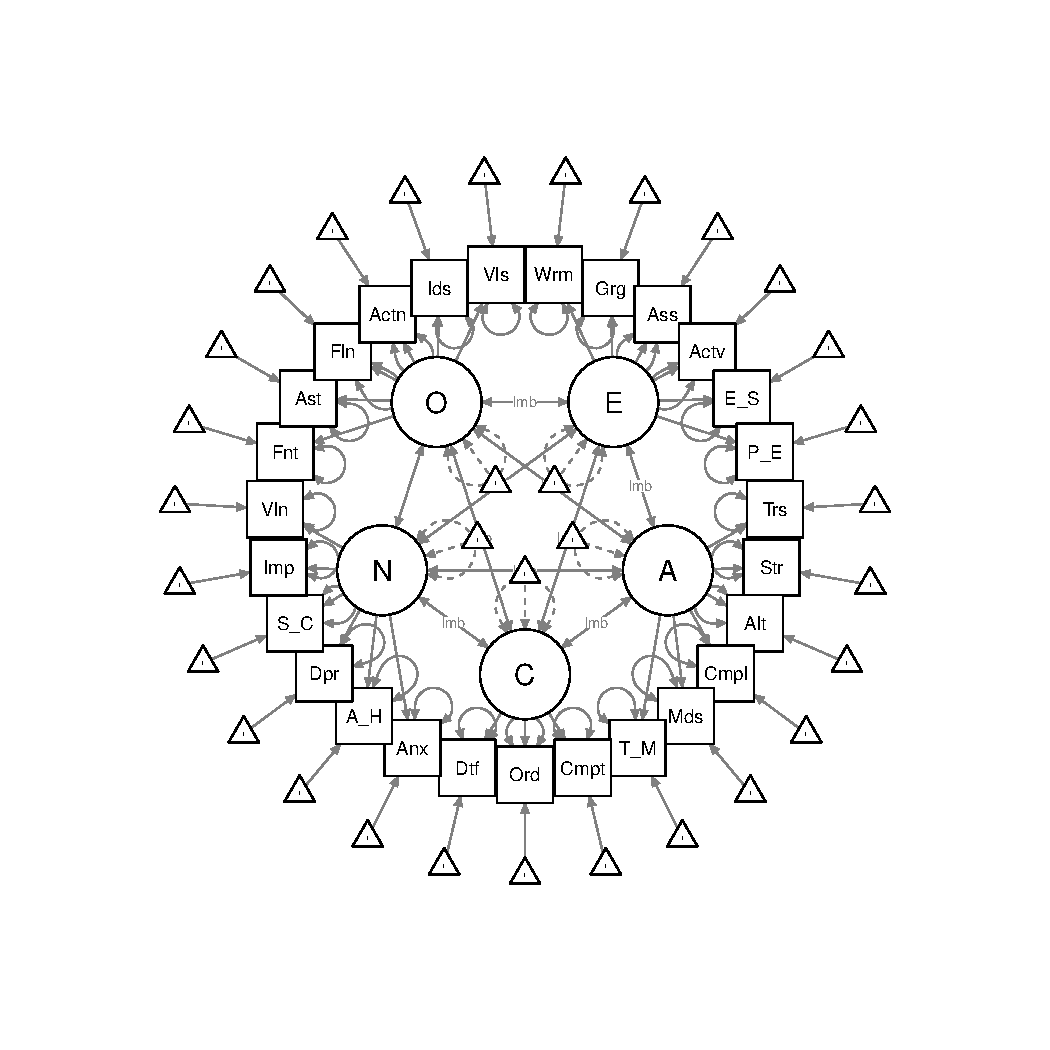
\includegraphics[width=\maxwidth]{figure/unnamed-chunk-8-1} 

\end{knitrout}

\subsection{Part A}
Is this constraint acceptable (i.e., is it statistically different from the model tested in Question 2)?
\begin{knitrout}
\definecolor{shadecolor}{rgb}{0.969, 0.969, 0.969}\color{fgcolor}\begin{kframe}
\begin{alltt}
\hlstd{(c3} \hlkwb{<-} \hlkwd{anova}\hlstd{(fit3, fit2))}
\end{alltt}
\begin{verbatim}
## Chi Square Difference Test
## 
##       Df    AIC    BIC  Chisq Chisq diff Df diff Pr(>Chisq)    
## fit2 314 9196.4 9497.0 1224.6                                  
## fit3 322 9323.4 9597.6 1367.6     143.04       8  < 2.2e-16 ***
## ---
## Signif. codes:  0 '***' 0.001 '**' 0.01 '*' 0.05 '.' 0.1 ' ' 1
\end{verbatim}
\end{kframe}
\end{knitrout}

Constraining the factor correlations to be equal does not appear to be justified, $\chi^2_{diff}(8) = 143.04$. 

\subsection{Part B}
Is the estimated latent variable correlation significant?

\begin{knitrout}
\definecolor{shadecolor}{rgb}{0.969, 0.969, 0.969}\color{fgcolor}\begin{kframe}
\begin{alltt}
\hlstd{res3} \hlkwb{<-} \hlkwd{parameterestimates}\hlstd{(fit3,} \hlkwc{standardized} \hlstd{= T)}

\hlstd{res3} \hlopt \hlstd{tbl_df} \hlopt \hlkwd{filter}\hlstd{(label} \hlopt{==} \hlstr{"lambda"}\hlstd{)} \hlopt
  \hlkwd{select}\hlstd{(label, est, ci.lower, ci.upper)} \hlopt
  \hlkwd{filter}\hlstd{(}\hlkwd{row_number}\hlstd{()} \hlopt{==} \hlnum{1}\hlstd{)}
\end{alltt}
\begin{verbatim}
## # A tibble: 1 x 4
##   label    est ci.lower ci.upper
##   <chr>  <dbl>    <dbl>    <dbl>
## 1 lambda 0.317    0.240    0.393
\end{verbatim}
\end{kframe}
\end{knitrout}

Yes, the estimated latent variable correlation is significant. 

\section{Question 4}
Use the most parsimonious model from the first three steps. Constrain the loadings within each dimension to be equal. Is this simplification acceptable?  

Fit 1 is the most parsimonious model because it estimates the fewest parameters.  

\begin{knitrout}
\definecolor{shadecolor}{rgb}{0.969, 0.969, 0.969}\color{fgcolor}\begin{kframe}
\begin{alltt}
\hlstd{b5.lc} \hlkwb{<-} \hlstr{'
# define the measurement model
E =~ lambdaE*Warmth + lambdaE*Gregariousness + lambdaE*Assertiveness + lambdaE*Activity + lambdaE*Excitement_Seeking + lambdaE*Positive_Emotions
A =~ lambdaA*Trust + lambdaA*Straightforwardness + lambdaA*Altruism + lambdaA*Compliance + lambdaA*Modesty + lambdaA*Tender_Mindedness
C =~ lambdaC*Competence + lambdaC*Order + lambdaC*Dutifulness + lambdaC*Competence + lambdaC*Order + lambdaC*Dutifulness
N =~ lambdaN*Anxiety + lambdaN*Angry_Hostility + lambdaN*Depression + lambdaN*Self_Consciousness + lambdaN*Impulsiveness + lambdaN*Vulnerability
O =~ lambdaO*Fantasy + lambdaO*Aesthetics + lambdaO*Feelings + lambdaO*Actions + lambdaO*Ideas + lambdaO*Values
'}

\hlstd{b5.mod} \hlkwb{<-} \hlkwd{paste}\hlstd{(b5.lc,} \hlstr{'\textbackslash{}n\textbackslash{}n'}\hlstd{, b5.uncorr,} \hlkwc{sep} \hlstd{=} \hlstr{''}\hlstd{,} \hlkwc{collapse} \hlstd{=} \hlstr{''}\hlstd{)}
\hlstd{fit4} \hlkwb{<-} \hlkwd{cfa}\hlstd{(b5.mod, dat,} \hlkwc{missing} \hlstd{=} \hlstr{'ML'}\hlstd{,} \hlkwc{std.lv} \hlstd{= T)}
\hlkwd{semPaths}\hlstd{(fit4,} \hlkwc{layout} \hlstd{=} \hlstr{"circle2"}\hlstd{)}
\end{alltt}
\end{kframe}
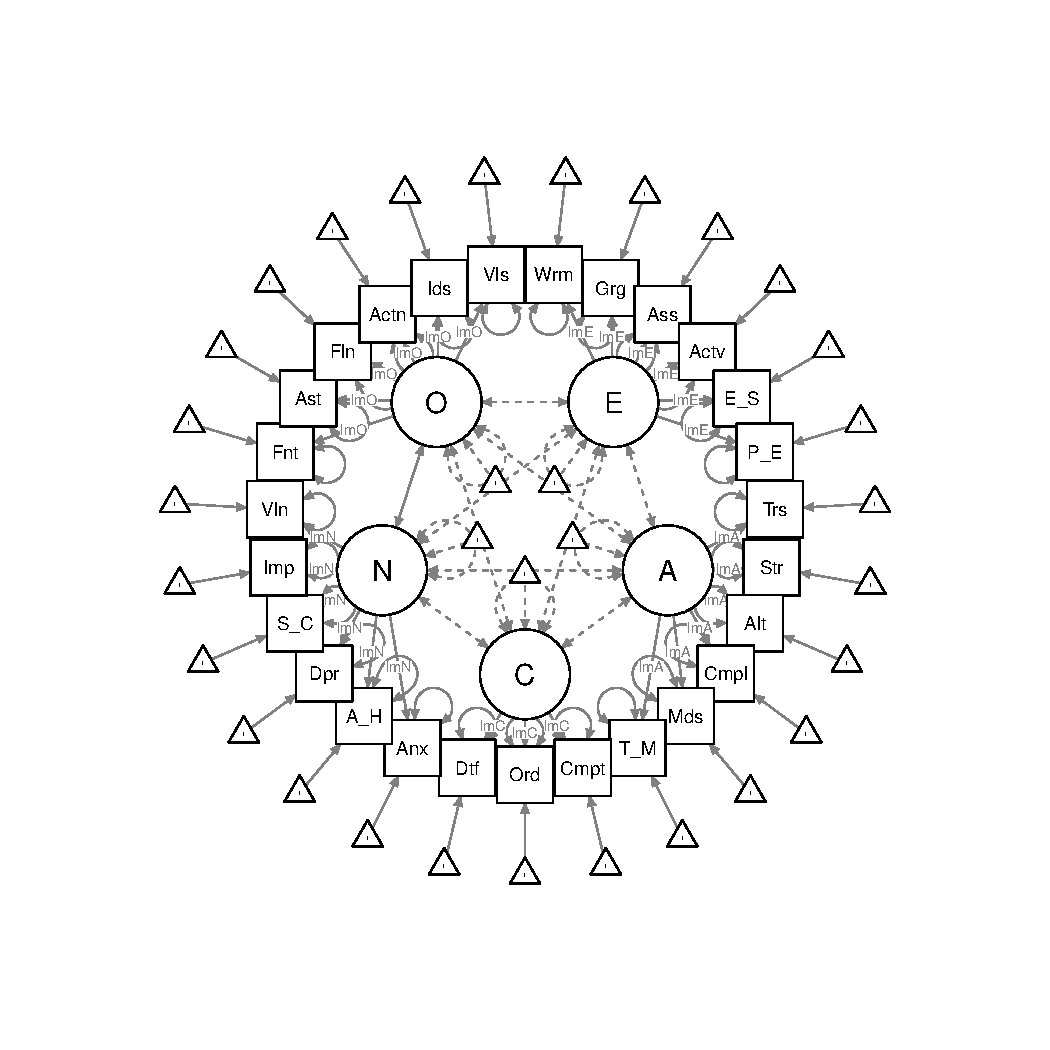
\includegraphics[width=\maxwidth]{figure/unnamed-chunk-11-1} 
\begin{kframe}\begin{alltt}
\hlkwd{summary}\hlstd{(fit4)}
\end{alltt}
\begin{verbatim}
## lavaan 0.6-3 ended normally after 53 iterations
## 
##   Optimization method                           NLMINB
##   Number of free parameters                         82
##   Number of equality constraints                    22
## 
##   Number of observations                           201
##   Number of missing patterns                         1
## 
##   Estimator                                         ML
##   Model Fit Test Statistic                    1617.926
##   Degrees of freedom                               345
##   P-value (Chi-square)                           0.000
## 
## Parameter Estimates:
## 
##   Information                                 Observed
##   Observed information based on                Hessian
##   Standard Errors                             Standard
## 
## Latent Variables:
##                    Estimate  Std.Err  z-value  P(>|z|)
##   E =~                                                
##     Warmth  (lmbE)    0.465    0.028   16.710    0.000
##     Grgrsns (lmbE)    0.465    0.028   16.710    0.000
##     Assrtvn (lmbE)    0.465    0.028   16.710    0.000
##     Activty (lmbE)    0.465    0.028   16.710    0.000
##     Exctm_S (lmbE)    0.465    0.028   16.710    0.000
##     Pstv_Em (lmbE)    0.465    0.028   16.710    0.000
##   A =~                                                
##     Trust   (lmbA)    0.402    0.025   16.166    0.000
##     Strghtf (lmbA)    0.402    0.025   16.166    0.000
##     Altrusm (lmbA)    0.402    0.025   16.166    0.000
##     Complnc (lmbA)    0.402    0.025   16.166    0.000
##     Modesty (lmbA)    0.402    0.025   16.166    0.000
##     Tndr_Mn (lmbA)    0.402    0.025   16.166    0.000
##   C =~                                                
##     Comptnc (lmbC)    0.495    0.031   15.921    0.000
##     Order   (lmbC)    0.495    0.031   15.921    0.000
##     Dtflnss (lmbC)    0.495    0.031   15.921    0.000
##   N =~                                                
##     Anxiety (lmbN)    0.531    0.031   17.238    0.000
##     Angry_H (lmbN)    0.531    0.031   17.238    0.000
##     Deprssn (lmbN)    0.531    0.031   17.238    0.000
##     Slf_Cns (lmbN)    0.531    0.031   17.238    0.000
##     Implsvn (lmbN)    0.531    0.031   17.238    0.000
##     Vlnrblt (lmbN)    0.531    0.031   17.238    0.000
##   O =~                                                
##     Fantasy (lmbO)    0.423    0.026   16.048    0.000
##     Asthtcs (lmbO)    0.423    0.026   16.048    0.000
##     Feelngs (lmbO)    0.423    0.026   16.048    0.000
##     Actions (lmbO)    0.423    0.026   16.048    0.000
##     Ideas   (lmbO)    0.423    0.026   16.048    0.000
##     Values  (lmbO)    0.423    0.026   16.048    0.000
## 
## Covariances:
##                    Estimate  Std.Err  z-value  P(>|z|)
##   E ~~                                                
##     A                 0.000                           
##     C                 0.000                           
##     N                 0.000                           
##     O                 0.000                           
##   A ~~                                                
##     C                 0.000                           
##     N                 0.000                           
##     O                 0.000                           
##   C ~~                                                
##     N                 0.000                           
##     O                 0.000                           
##   N ~~                                                
##     O                 0.203    0.082    2.478    0.013
## 
## Intercepts:
##                    Estimate  Std.Err  z-value  P(>|z|)
##    .Warmth            3.780    0.045   84.907    0.000
##    .Gregariousness    3.158    0.049   63.972    0.000
##    .Assertiveness     2.942    0.052   57.043    0.000
##    .Activity          3.229    0.044   72.811    0.000
##    .Excitemnt_Skng    3.585    0.049   72.695    0.000
##    .Positive_Emtns    3.684    0.048   76.864    0.000
##    .Trust             3.343    0.048   70.259    0.000
##    .Strghtfrwrdnss    3.248    0.048   67.059    0.000
##    .Altruism          3.897    0.040   97.411    0.000
##    .Compliance        3.115    0.044   70.167    0.000
##    .Modesty           3.161    0.048   66.373    0.000
##    .Tender_Mnddnss    3.511    0.040   87.448    0.000
##    .Competence        3.486    0.044   80.074    0.000
##    .Order             3.166    0.052   60.365    0.000
##    .Dutifulness       3.630    0.045   80.644    0.000
##    .Anxiety           3.384    0.049   68.746    0.000
##    .Angry_Hostilty    2.822    0.055   51.059    0.000
##    .Depression        2.950    0.052   57.271    0.000
##    .Self_Conscsnss    3.111    0.048   64.762    0.000
##    .Impulsiveness     3.250    0.054   60.204    0.000
##    .Vulnerability     2.610    0.047   55.506    0.000
##    .Fantasy           3.660    0.048   75.811    0.000
##    .Aesthetics        3.364    0.056   59.660    0.000
##    .Feelings          3.887    0.047   82.656    0.000
##    .Actions           2.971    0.043   68.458    0.000
##    .Ideas             3.514    0.055   64.438    0.000
##    .Values            3.784    0.041   93.083    0.000
##     E                 0.000                           
##     A                 0.000                           
##     C                 0.000                           
##     N                 0.000                           
##     O                 0.000                           
## 
## Variances:
##                    Estimate  Std.Err  z-value  P(>|z|)
##    .Warmth            0.182    0.023    8.010    0.000
##    .Gregariousness    0.274    0.031    8.757    0.000
##    .Assertiveness     0.318    0.036    8.957    0.000
##    .Activity          0.179    0.022    8.047    0.000
##    .Excitemnt_Skng    0.272    0.031    8.728    0.000
##    .Positive_Emtns    0.245    0.029    8.544    0.000
##    .Trust             0.293    0.033    8.938    0.000
##    .Strghtfrwrdnss    0.309    0.034    9.000    0.000
##    .Altruism          0.160    0.020    8.049    0.000
##    .Compliance        0.234    0.027    8.695    0.000
##    .Modesty           0.294    0.033    8.956    0.000
##    .Tender_Mnddnss    0.162    0.020    8.097    0.000
##    .Competence        0.136    0.022    6.253    0.000
##    .Order             0.308    0.037    8.379    0.000
##    .Dutifulness       0.163    0.024    6.824    0.000
##    .Anxiety           0.205    0.025    8.258    0.000
##    .Angry_Hostilty    0.332    0.037    8.919    0.000
##    .Depression        0.252    0.029    8.592    0.000
##    .Self_Conscsnss    0.182    0.022    8.097    0.000
##    .Impulsiveness     0.304    0.035    8.714    0.000
##    .Vulnerability     0.163    0.021    7.911    0.000
##    .Fantasy           0.290    0.033    8.773    0.000
##    .Aesthetics        0.460    0.050    9.232    0.000
##    .Feelings          0.266    0.031    8.644    0.000
##    .Actions           0.200    0.024    8.211    0.000
##    .Ideas             0.419    0.046    9.171    0.000
##    .Values            0.154    0.020    7.723    0.000
##     E                 1.000                           
##     A                 1.000                           
##     C                 1.000                           
##     N                 1.000                           
##     O                 1.000
\end{verbatim}
\begin{alltt}
\hlstd{(c4} \hlkwb{<-} \hlkwd{anova}\hlstd{(fit1, fit4))}
\end{alltt}
\begin{verbatim}
## Chi Square Difference Test
## 
##       Df    AIC    BIC  Chisq Chisq diff Df diff Pr(>Chisq)    
## fit1 324 9419.2 9686.8 1467.5                                  
## fit4 345 9527.7 9725.9 1617.9     150.46      21  < 2.2e-16 ***
## ---
## Signif. codes:  0 '***' 0.001 '**' 0.01 '*' 0.05 '.' 0.1 ' ' 1
\end{verbatim}
\end{kframe}
\end{knitrout}

A likelihood ratio test suggests that constraining the loadings is not justified. $\chi^2_{diff}(21) = 150.46$

\section{Question 5}
Use the modification indices to diagnose the major problem with the model in Question 2. What change to that model would produce the biggest improvement in model fit?
\begin{knitrout}
\definecolor{shadecolor}{rgb}{0.969, 0.969, 0.969}\color{fgcolor}\begin{kframe}
\begin{alltt}
\hlstd{mi2} \hlkwb{<-} \hlkwd{modificationindices}\hlstd{(fit2)} \hlopt \hlkwd{arrange}\hlstd{(}\hlkwd{desc}\hlstd{(mi))}
\end{alltt}
\end{kframe}
\end{knitrout}

The biggest problem in the model from Question 2 was the $covariation$ between $Compliance Angry_Hostility$. 


\end{document}
